\documentclass[aps,pra,twocolumn,superscriptaddress,nofootinbib,longbibliography]{revtex4-2}

\usepackage{amsmath,amssymb}
\usepackage{physics}
\usepackage{dsfont}
\usepackage{bm}
\usepackage{graphicx}
\usepackage[dvipsnames]{xcolor}
\usepackage{tikz}
\usetikzlibrary{arrows.meta,positioning,shapes.geometric,calc,fit,backgrounds}
\usepackage{quantikz}
\usepackage{booktabs}
\usepackage[colorlinks=true,allcolors=RoyalBlue]{hyperref}

\graphicspath{{figures/}}

\DeclareMathOperator{\vecc}{vec}
\newcommand{\id}{\mathds{1}}
\newcommand{\rhoS}{\rho_{S}}
\newcommand{\Ldt}{\mathcal{L}}
\newcommand{\Emap}{\mathcal{E}}
\newcommand{\Lmap}{\mathrm{L}}
\newcommand{\dt}{\Delta t}
\newcommand{\cm}{\,\mathrm{cm}^{-1}}

\tikzset{
  stage/.style={draw,rounded corners=2pt,align=center,inner sep=3pt,
    font=\footnotesize,minimum height=8mm,fill=Gray!8},
  qpu/.style={draw,rounded corners=2pt,align=center,inner sep=3pt,
    font=\footnotesize,minimum height=8mm,fill=RoyalBlue!12},
  flow/.style={-{Stealth[length=2mm]},thick},
  recyc/.style={-{Stealth[length=2mm]},thick,RoyalBlue},
}

\begin{document}

\title{Putting open-system dynamics on a quantum grid\\
transfer tensors bring the non-Markovian memory onto the register}

\author{Simon Mader}
\email{simon.mader@jku.at}
\affiliation{Institute for Theoretical Physics, Johannes Kepler University Linz, Altenberger Stra\ss{}e 69, 4040 Linz, Austria}
\author{Akhil Bhartiya}
\affiliation{Institute for Theoretical Physics, Johannes Kepler University Linz, Altenberger Stra\ss{}e 69, 4040 Linz, Austria}
\author{Tobias Kramer}
\affiliation{Institute for Theoretical Physics, Johannes Kepler University Linz, Altenberger Stra\ss{}e 69, 4040 Linz, Austria}

\date{\today}

\begin{abstract}
Simulating open quantum systems on quantum hardware is obstructed by a basic
mismatch. Dissipative dynamics is non-unitary, while a quantum circuit
implements only unitary operations. Dilation based schemes embed the dynamical
map into a larger unitary and resolve this in principle, yet existing
implementations rebuild the map for every time step and leave almost all of the
work on the classical computer. We place the propagator on a grid instead. The
dynamical map is turned once into a single dilated unitary, and the quantum
computer generates the whole trajectory by re-applying that one circuit, reading
the state out and feeding it back. For Markovian dynamics the Lindblad map is a
semigroup, so one set of Kraus operators for a single step is enough. A
non-Markovian map is not a semigroup, and a channel acting on the system alone
cannot carry memory. We therefore place the memory on the register. The exact
dynamics is written as a discrete convolution over transfer tensors, which decay
once the bath forgets, so only the tensors inside a finite memory window need to
be learned. They are packed into one fixed companion operator that advances a
sliding window of past states, and its Sz.-Nagy dilation is the single reused
circuit. The classical cost then covers only the memory time and not the full
propagation. We demonstrate the method on a four-site Fenna-Matthews-Olson
pathway with three independently computed maps, the Lindblad equation, the
hierarchical equations of motion, and a tensor-network path integral, and
reproduce the numerically exact dynamics to 1000 fs from a memory window of 150
to 250 fs. Discarding the memory returns an error of order one, which shows that
the window is essential. The bulk of a non-Markovian open-system simulation is
thereby carried out on the quantum device.
\end{abstract}

\maketitle

% ==========================================================================
\section{Introduction}
\label{sec:intro}
% ==========================================================================
An open quantum system is a system of interest that cannot be isolated from its
environment. The coupling to that environment produces decoherence, dissipation
and energy transport, effects that are central to chemistry, condensed-matter
physics and quantum technology~\cite{breuer2002}. A prominent example is the
Fenna-Matthews-Olson (FMO) pigment-protein complex, which guides electronic
excitations toward a reaction center with almost unit efficiency and in which
long-lived coherences have been observed at physiological
temperature~\cite{fenna1975,engel2007,ishizaki2009,adolphs2006}. On a classical
computer the joint system-bath Hilbert space grows exponentially, which makes
numerically exact simulation expensive, and the non-Markovian regime, in which
the bath keeps a memory of the past, is the hardest part~\cite{seneviratne2024}.
Feynman and Lloyd argued that a controllable quantum device could carry out such
simulations more naturally~\cite{feynman1982,lloyd1996}, and this promise drives
the search for open-system algorithms that run on today's
hardware~\cite{preskill2018}.

The obstacle is structural. The reduced dynamics of an open system is
non-unitary, whereas a quantum circuit realizes only unitary
operations~\cite{nielsen2010}. Several schemes address Markovian dissipation on
a device~\cite{sweke2015,kliesch2011,cleve2017,schlimgen2021}, and the most
direct route uses dilation. In a dilation the Kraus operators of the dynamical
map are embedded into a larger unitary that acts on the system together with one
ancilla, and the physical output is read from a subspace of the enlarged
register~\cite{hu2022,seneviratne2024}. This makes open-system dynamics
implementable on hardware and has been demonstrated for the FMO complex on NISQ
devices~\cite{hu2022,seneviratne2024,headmarsden2021}.

These schemes, however, rebuild the map for every output time. To reach a time
$t$ the Kraus operators are reconstructed from scratch at each step through a
Choi decomposition, a singular value decomposition and a dilation, and all of
this runs classically. The circuit is executed only afterwards, once the answer
is effectively already known, so the classical effort grows with the length of
the propagation and the quantum device barely contributes.

We remove this repetition by putting the propagator on a grid, sketched in
Fig.~\ref{fig:reuse}. The classical side produces one operator, that operator is
turned once into a single dilated unitary, and the quantum computer generates
the entire trajectory by re-applying the same circuit, reading the state out
after each step and feeding it back as the next input. Which operator plays this
role depends on the memory of the dynamics. For a Markovian map the Lindblad
generator is time independent, so the map is a semigroup and a single one-step
propagator suffices. A non-Markovian map is not a semigroup. A channel acting on
the system alone, applied over and over, can only ever produce a semigroup, so
it necessarily discards every correlation older than one step. We keep the
memory by enlarging the register. Writing the exact dynamics as a discrete
convolution over transfer tensors~\cite{cerrillo2014}, which decay once the bath
forgets, only the tensors inside a finite memory window survive. They are
collected into one fixed companion operator that advances a sliding window of
past states, and the Sz.-Nagy dilation of that operator is the single reused
circuit. The classical cost then covers only the memory time and not the full
propagation, in contrast to the per-step reconstruction of the earlier schemes.

\begin{figure}[t]
\centering
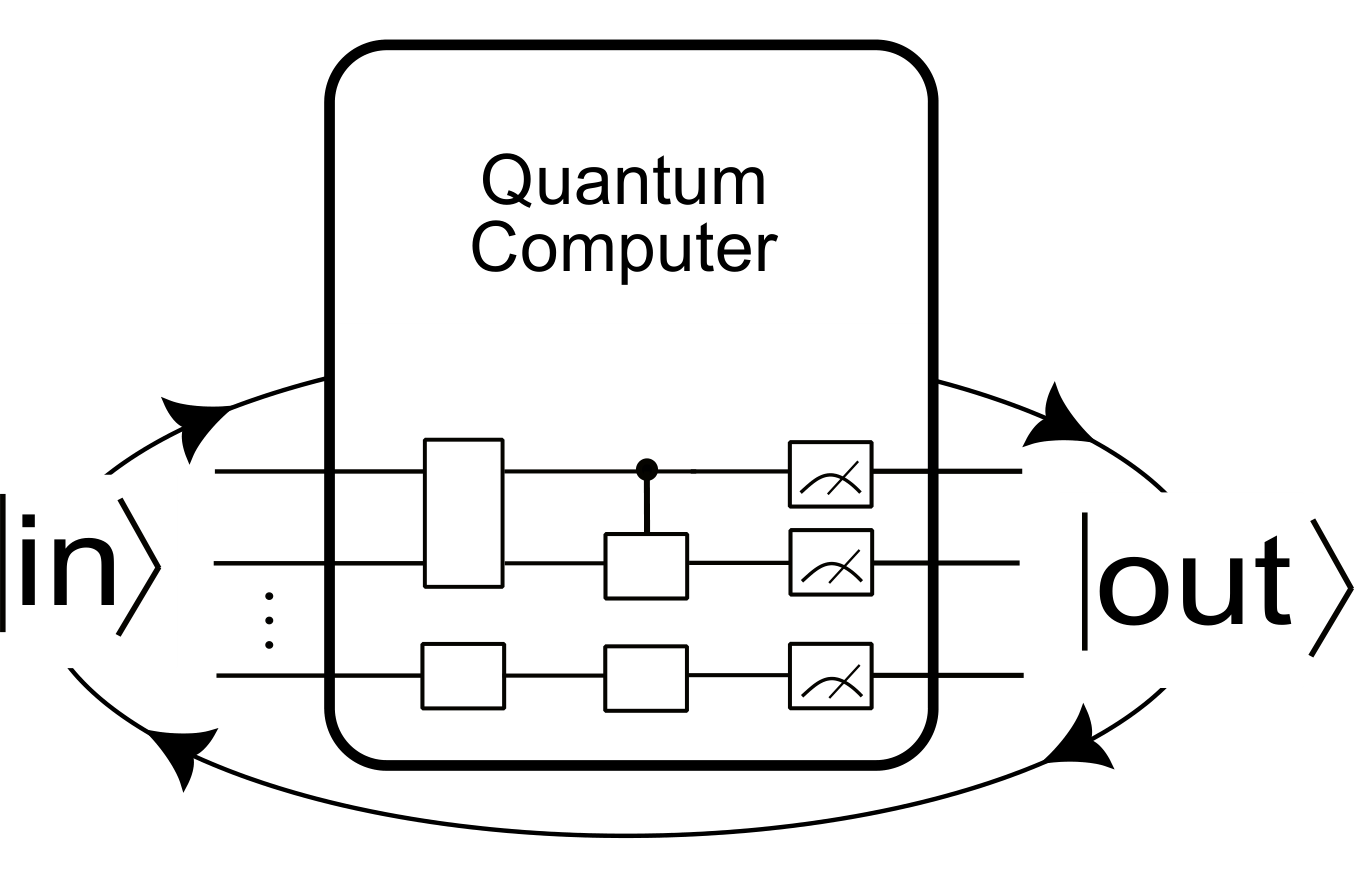
\includegraphics[width=0.86\columnwidth]{proposal_reuse.png}
\caption{\label{fig:reuse}
The grid. One operator, built once on the classical side, becomes a single
circuit that the quantum computer re-applies at every step. The output state is
read out and fed back as the next input, so no operator is recomputed during the
propagation. Figure adapted from the authors' research proposal.}
\end{figure}

We build all three of the maps that feed this grid, the Lindblad equation, the
hierarchical equations of motion (HEOM)~\cite{tanimura1989,tanimura2020}, and a
tensor-network path integral~\cite{strathearn2018,bose2022}, for a four-site FMO
pathway, and reproduce the numerically exact dynamics to 1000 fs from a single
reused circuit whose classical input reaches only 150 to 250 fs. The paper is
organized as follows. Section~\ref{sec:map} casts the dynamics as a family of
linear maps and lists the three sources. Section~\ref{sec:markov} puts the
Markovian map on the grid. Section~\ref{sec:memory} develops the memory window
and the transfer-tensor construction that carries the non-Markovian case.
Section~\ref{sec:results} presents the FMO results, and
Secs.~\ref{sec:outlook} and \ref{sec:conclusion} give the outlook and the
conclusion. Three appendices collect the vectorization and Choi-Kraus
construction, the transfer-tensor derivation, and a comparison with the earlier
schemes.

% ==========================================================================
\section{Open-system dynamics as a family of maps}
\label{sec:map}
% ==========================================================================
The total Hamiltonian reads $H=H_S+H_B+H_{SB}$, with a system, a bath and an
interaction term. The object of interest is the reduced density matrix
$\rhoS(t)=\Tr_B[\rho(t)]$. For a factorized initial condition
$\rho(0)=\rhoS(0)\otimes\rho_B$ its evolution is a family of linear, completely
positive and trace-preserving (CPTP) maps~\cite{breuer2002,nielsen2010},
\begin{equation}
  \label{eq:dynmap}
  \rhoS(t_n)=\Emap_n[\rhoS(0)],\qquad t_n=n\dt,
\end{equation}
one map for each point of a uniform time grid of spacing $\dt$. Stacking the
columns of the density matrix into the vector $\vecc(\rhoS)$ turns every map into
a matrix, and Eq.~\eqref{eq:dynmap} becomes
\begin{equation}
  \label{eq:vecmap}
  \vecc\!\big(\rhoS(t_n)\big)=\Lmap_n\,\vecc\!\big(\rhoS(0)\big),
\end{equation}
where $\Lmap_n$ is the $d^2\times d^2$ matrix of $\Emap_n$ for a system of
dimension $d$. The family $\{\Lmap_n\}$ is the single input to everything that
follows. Its completely positive and trace-preserving character is all that is
used, and the physical origin of the maps never enters.

For the four-site FMO pathway the system carries one excitation shared among
$d=4$ sites. The system Hamiltonian in the site basis, in wavenumbers and
relative to its mean, is~\cite{seneviratne2024}
\begin{equation}
  \label{eq:H}
  H_S=\begin{pmatrix}
   42.5 & -87.7 & 5.5 & -5.9\\
  -87.7 & 162.5 & 30.8 & 8.2\\
   5.5 & 30.8 & -157.5 & -53.4\\
  -5.9 & 8.2 & -53.4 & -47.5
  \end{pmatrix}\cm,
\end{equation}
where the diagonal entries are the site energies and the off-diagonal entries the
dipole couplings. Each site couples to an independent phonon bath with the
Drude-Lorentz spectral density
\begin{equation}
  \label{eq:J}
  J(\omega)=\frac{2\lambda\gamma\,\omega}{\omega^{2}+\gamma^{2}},
\end{equation}
of reorganization energy $\lambda=35\cm$ and cutoff $\gamma=106.18\cm$ at
temperature $T=300$~K. The bath enters only through its correlation function
\begin{equation}
  \label{eq:Ctau}
  C(\tau)=\frac{1}{\pi}\int_0^\infty\!\!d\omega\,J(\omega)\Big[\coth\tfrac{\hbar\omega}{2k_BT}\cos\omega\tau-i\sin\omega\tau\Big],
\end{equation}
which feeds the influence functional of the path integral, the exponential
expansion of the HEOM, and the rates of the Lindblad generator alike.

We obtain the family from three independent methods, each numerically exact
within its own approximation and each established in the literature. A fuller
account of how each map is built is given in Appendix~\ref{app:maps}.

\emph{Lindblad.} In the Markovian limit the reduced dynamics obeys the Lindblad
master equation~\cite{lindblad1976,gks1976}, whose generator is written out in
Appendix~\ref{app:vec}. Its dissipation rates and jump operators follow from the
spectral density through the secular Redfield construction. The generator $\Ldt$
is time independent, so $\Lmap_n=e^{\Ldt t_n}=\Lmap_1^{\,n}$ and the family is a
quantum dynamical semigroup.

\emph{Hierarchical equations of motion.} The HEOM are a numerically exact,
non-perturbative treatment of a Gaussian bath~\cite{tanimura1989,tanimura2020}.
The correlation function is written as a sum of exponentials
$C(\tau)=\sum_k c_k e^{-\nu_k\tau}$, and the reduced density matrix
$\rhoS=\rho_{\bm 0}$ is embedded as the lowest member of a hierarchy of auxiliary
density operators $\rho_{\bm n}$, labeled by a multi-index $\bm n$, that satisfy
\begin{equation}
  \label{eq:heom}
  \begin{split}
  \dot\rho_{\bm n}=&-\Big(\tfrac{i}{\hbar}[H_S,\cdot]+\sum_k n_k\nu_k\Big)\rho_{\bm n}\\
  &-i\sum_k\Big([V,\rho_{\bm n_k^+}]+n_k\big(c_k V\rho_{\bm n_k^-}-c_k^*\rho_{\bm n_k^-}V\big)\Big),
  \end{split}
\end{equation}
with $V$ the system-bath coupling and $\bm n_k^\pm$ the multi-index with its
$k$th entry raised or lowered. Truncating at a finite depth collects the right
hand side into one extended Liouvillian $\hat\Ldt_{\rm HEOM}$, and the single
matrix exponential $P=e^{\hat\Ldt_{\rm HEOM}\dt}$ advances the full hierarchy by
one step. Propagating a complete set of system matrices and reading off
$\rho_{\bm 0}$ yields the reduced maps $\Lmap_n$.

\emph{Tensor-network path integral.} The reduced dynamics equally follows from
the real-time path integral over the forward and backward system paths
$s^\pm(t)$~\cite{feynmanvernon1963},
\begin{equation}
  \label{eq:pathint}
  \begin{split}
  \rhoS(s_t^+,s_t^-)=\int\!\mathcal{D}s^+\!\!\int\!\mathcal{D}s^-\;
  &\bra{s_0^+}\rhoS(0)\ket{s_0^-}\\[-1pt]
  &\times e^{\frac{i}{\hbar}(S[s^+]-S[s^-])}\,I_F[s^+,s^-],
  \end{split}
\end{equation}
where $S[s]$ is the bare system action and the entire effect of the bath is
carried by the Feynman-Vernon influence functional. On the discretized contour,
with slice labels $s_k^\pm$, it is the pairwise product~\cite{makri1995}
\begin{equation}
  \label{eq:influence}
  I_F=\exp\!\Big\{\!-\tfrac1\hbar\sum_{k}\sum_{k'\le k}(s_k^+-s_k^-)\big(\eta_{kk'}s_{k'}^+-\eta_{kk'}^*s_{k'}^-\big)\Big\},
\end{equation}
whose coefficients $\eta_{kk'}$ are double time integrals of $C(\tau)$ over the
slices. The augmented path-amplitude tensor is contracted as a matrix product
state in the TEMPO manner~\cite{strathearn2018,bose2022}, and keeping the initial
forward-backward index open returns the family $\Lmap_n$ directly.

The Lindblad family is a semigroup and is placed on the grid in
Sec.~\ref{sec:markov}. The HEOM and path-integral families are not, and are
handled in Sec.~\ref{sec:memory}.

% ==========================================================================
\section{The Markovian grid}
\label{sec:markov}
% ==========================================================================
The grid follows the workflow of Fig.~\ref{fig:workflow}. A dynamical map, from
any of the three sources, is decomposed once into the operators that the circuit
reuses, the circuit is dilated a single time, and the vectorized density matrix
returned by one run initializes the next. For a Markovian map, treated in this
section, these operators are the one-step Kraus operators; for a non-Markovian
map they are replaced by the single companion operator of Sec.~\ref{sec:memory}.

\begin{figure}[t]
\centering
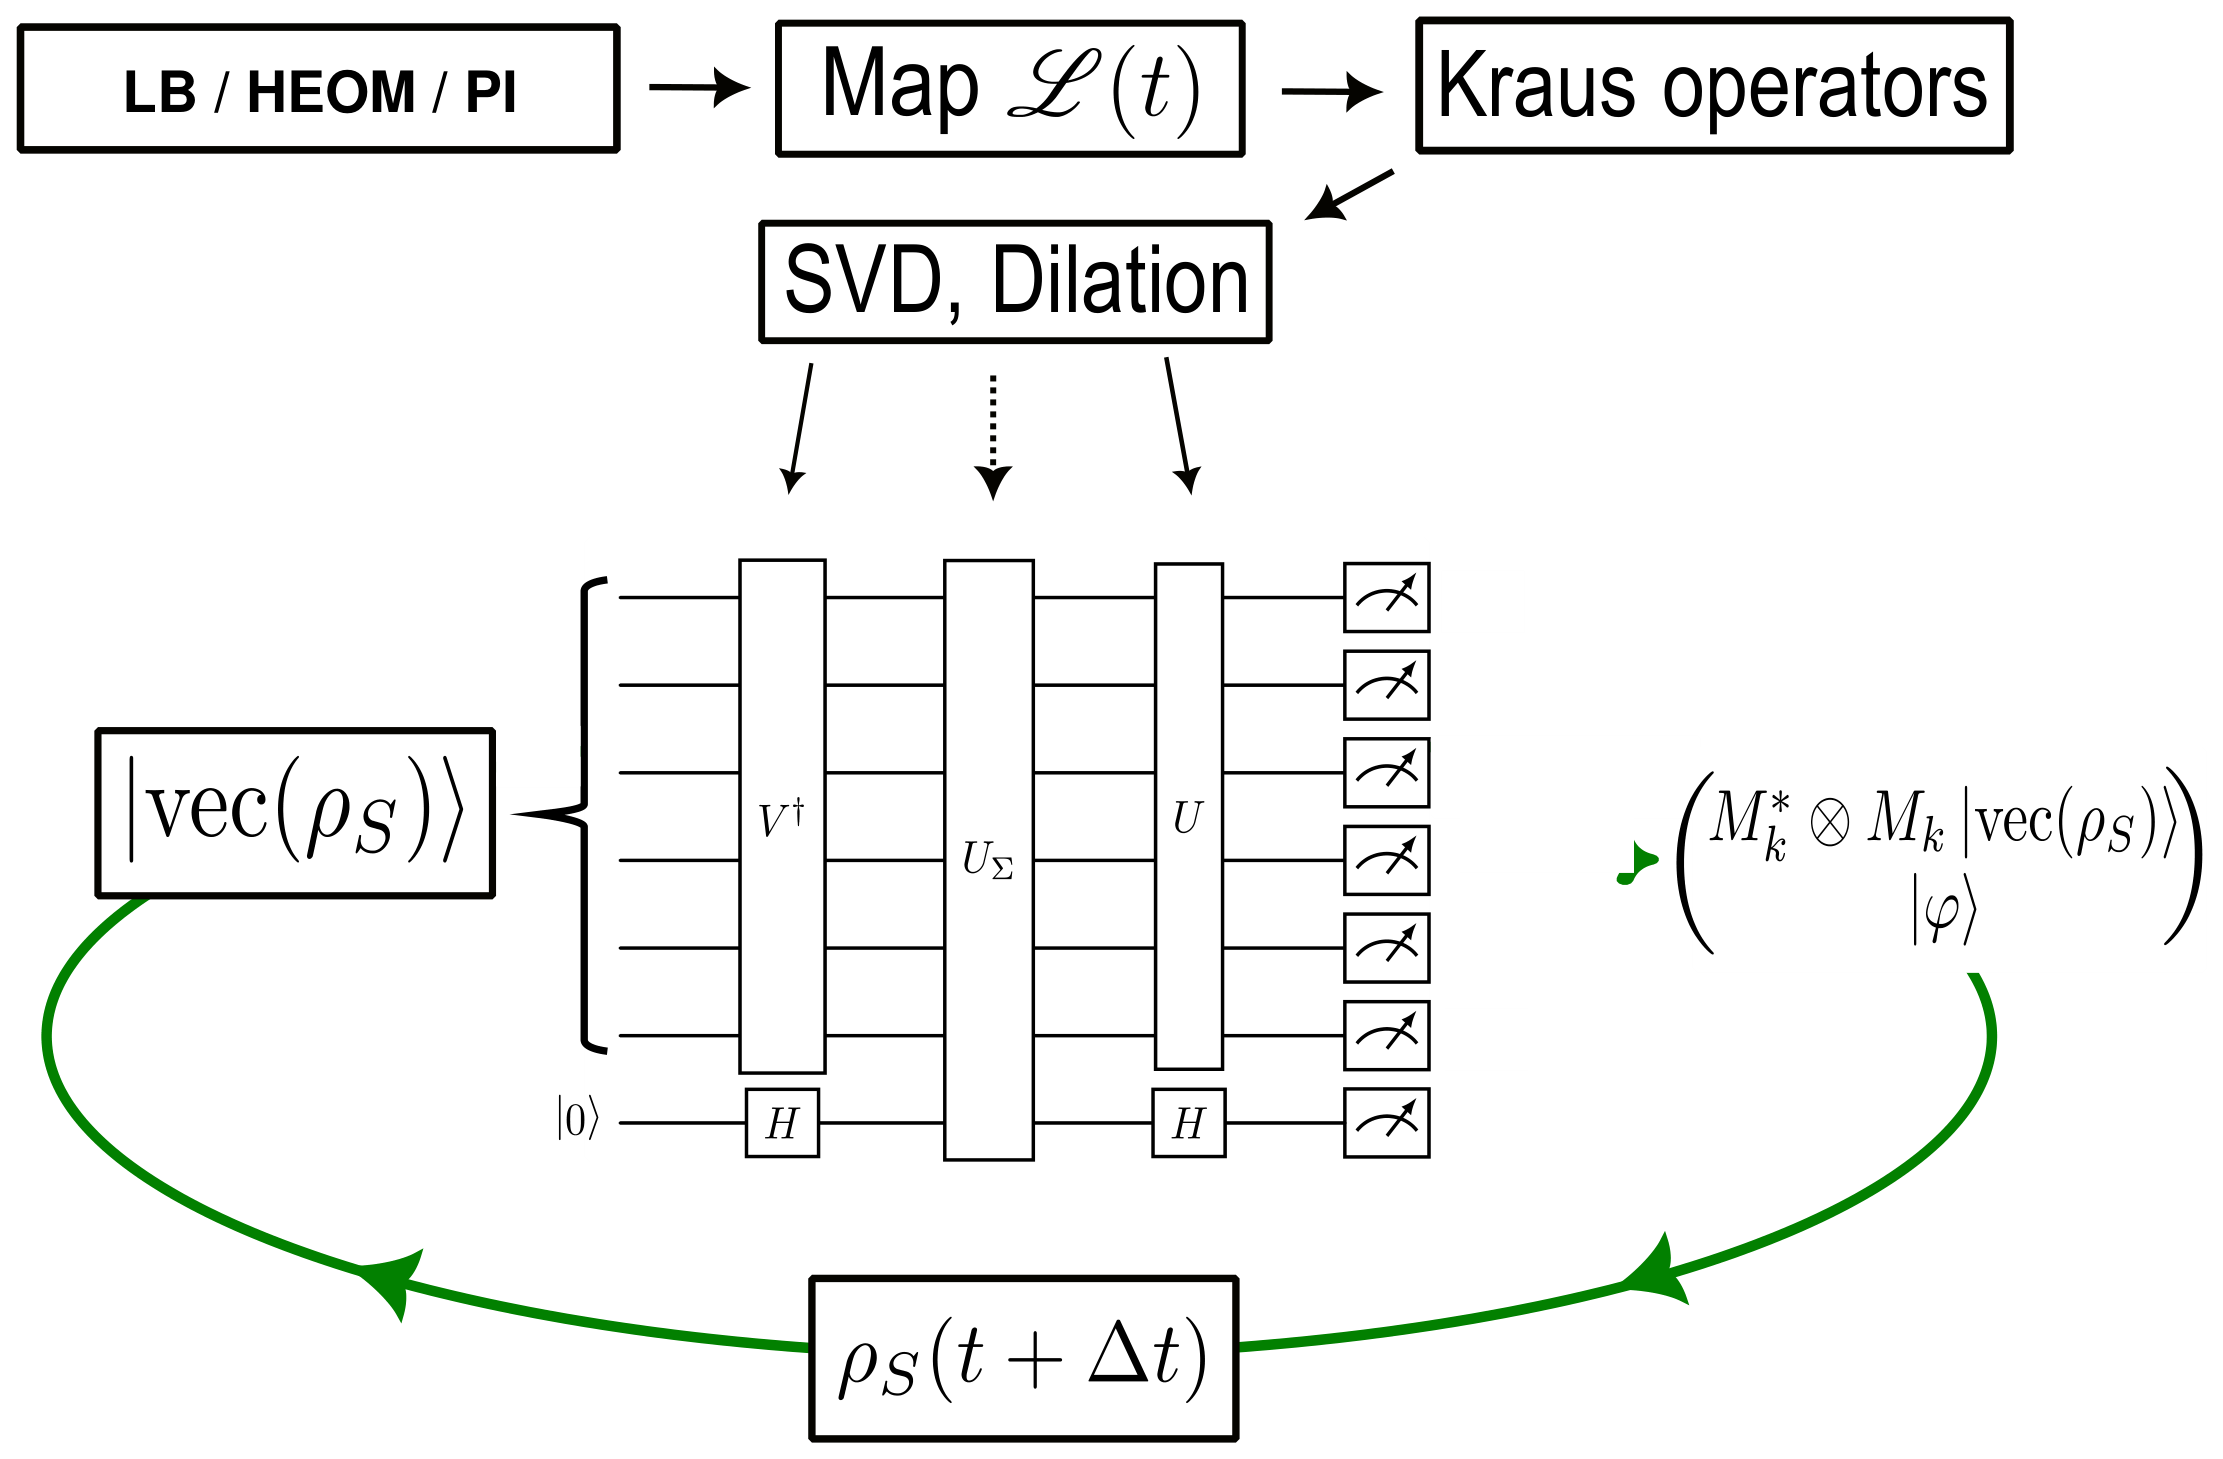
\includegraphics[width=\columnwidth]{enh_workflow.png}
\caption{\label{fig:workflow}
Workflow of the grid. A map from the Lindblad equation, the HEOM or the path
integral (LB / HEOM / PI) is turned once into the operators the circuit reuses,
which are dilated into the circuit shown ($V^\dagger$, $U_\Sigma$, $U$ with the
ancilla Hadamards realize the dilation, here in its singular-value form). The
circuit acts on $\ket{\vecc\rhoS}$, and its output $\rhoS(t+\dt)$ is fed back
along the green loop, so the propagation runs on the quantum device. Figure
adapted from the authors' research proposal.}
\end{figure}

When the family is a semigroup, a single map carries all of it. From
$\Lmap_n=\Lmap_1^{\,n}$ the propagation is
\begin{equation}
  \label{eq:markstep}
  \rhoS(t_{n})=\sum_k M_k\,\rhoS(t_{n-1})\,M_k^\dagger,
\end{equation}
with one fixed set of Kraus operators $M_k$ of the one-step map $\Lmap_1$. They
follow from the Choi decomposition of $\Lmap_1$ (Appendix~\ref{app:vec}), which
is performed once. To iterate Eq.~\eqref{eq:markstep} on a circuit the state
$\rhoS(t_{n-1})$ must be loaded at each step. A pure state would be loaded as a
vector, but decoherence makes $\rhoS$ mixed, and no state vector represents a
mixed density matrix. We therefore load the vectorized density matrix. Using
$\vecc(M\rhoS M^\dagger)=(M^{*}\otimes M)\vecc(\rhoS)$, Eq.~\eqref{eq:markstep}
reads
\begin{equation}
  \label{eq:markvec}
  \vecc\!\big(\rhoS(t_{n})\big)=\sum_k\big(M_k^{*}\otimes M_k\big)\,
  \vecc\!\big(\rhoS(t_{n-1})\big).
\end{equation}
Each $M_k^{*}\otimes M_k$ is a contraction, so it becomes the top-left block of a
unitary one qubit larger through the Sz.-Nagy dilation~\cite{sznagy2010}
\begin{equation}
  \label{eq:sznagy}
  U_A=\begin{pmatrix}A & \sqrt{\id-AA^\dagger}\\ \sqrt{\id-A^\dagger A} & -A^\dagger\end{pmatrix},
  \qquad A=\tfrac{1}{s}\,M_k^{*}\otimes M_k,
\end{equation}
with a scale $s\ge\|A\|$ that is undone classically after read-out. Preparing
$\ket{0}_{\rm anc}\otimes\ket{\vecc\rhoS}$, applying $U_A$ and post-selecting the
ancilla on $\ket{0}$ leaves $A\ket{\vecc\rhoS}$ in the first register, which is
one term of Eq.~\eqref{eq:markvec}. Running the circuit of
Fig.~\ref{fig:circuits} for each Kraus operator and summing the outputs gives
$\vecc(\rhoS(t_n))$, which initializes the next step. This operator sum and the
recycling are drawn in Fig.~\ref{fig:opsum}. The circuits are built once and
re-applied, so the entire Markovian trajectory follows from a single classical
dilation. For the four-site model $\vecc(\rhoS)$ has $16$ amplitudes, which is
four system qubits and one ancilla.

\begin{figure*}[t]
\centering
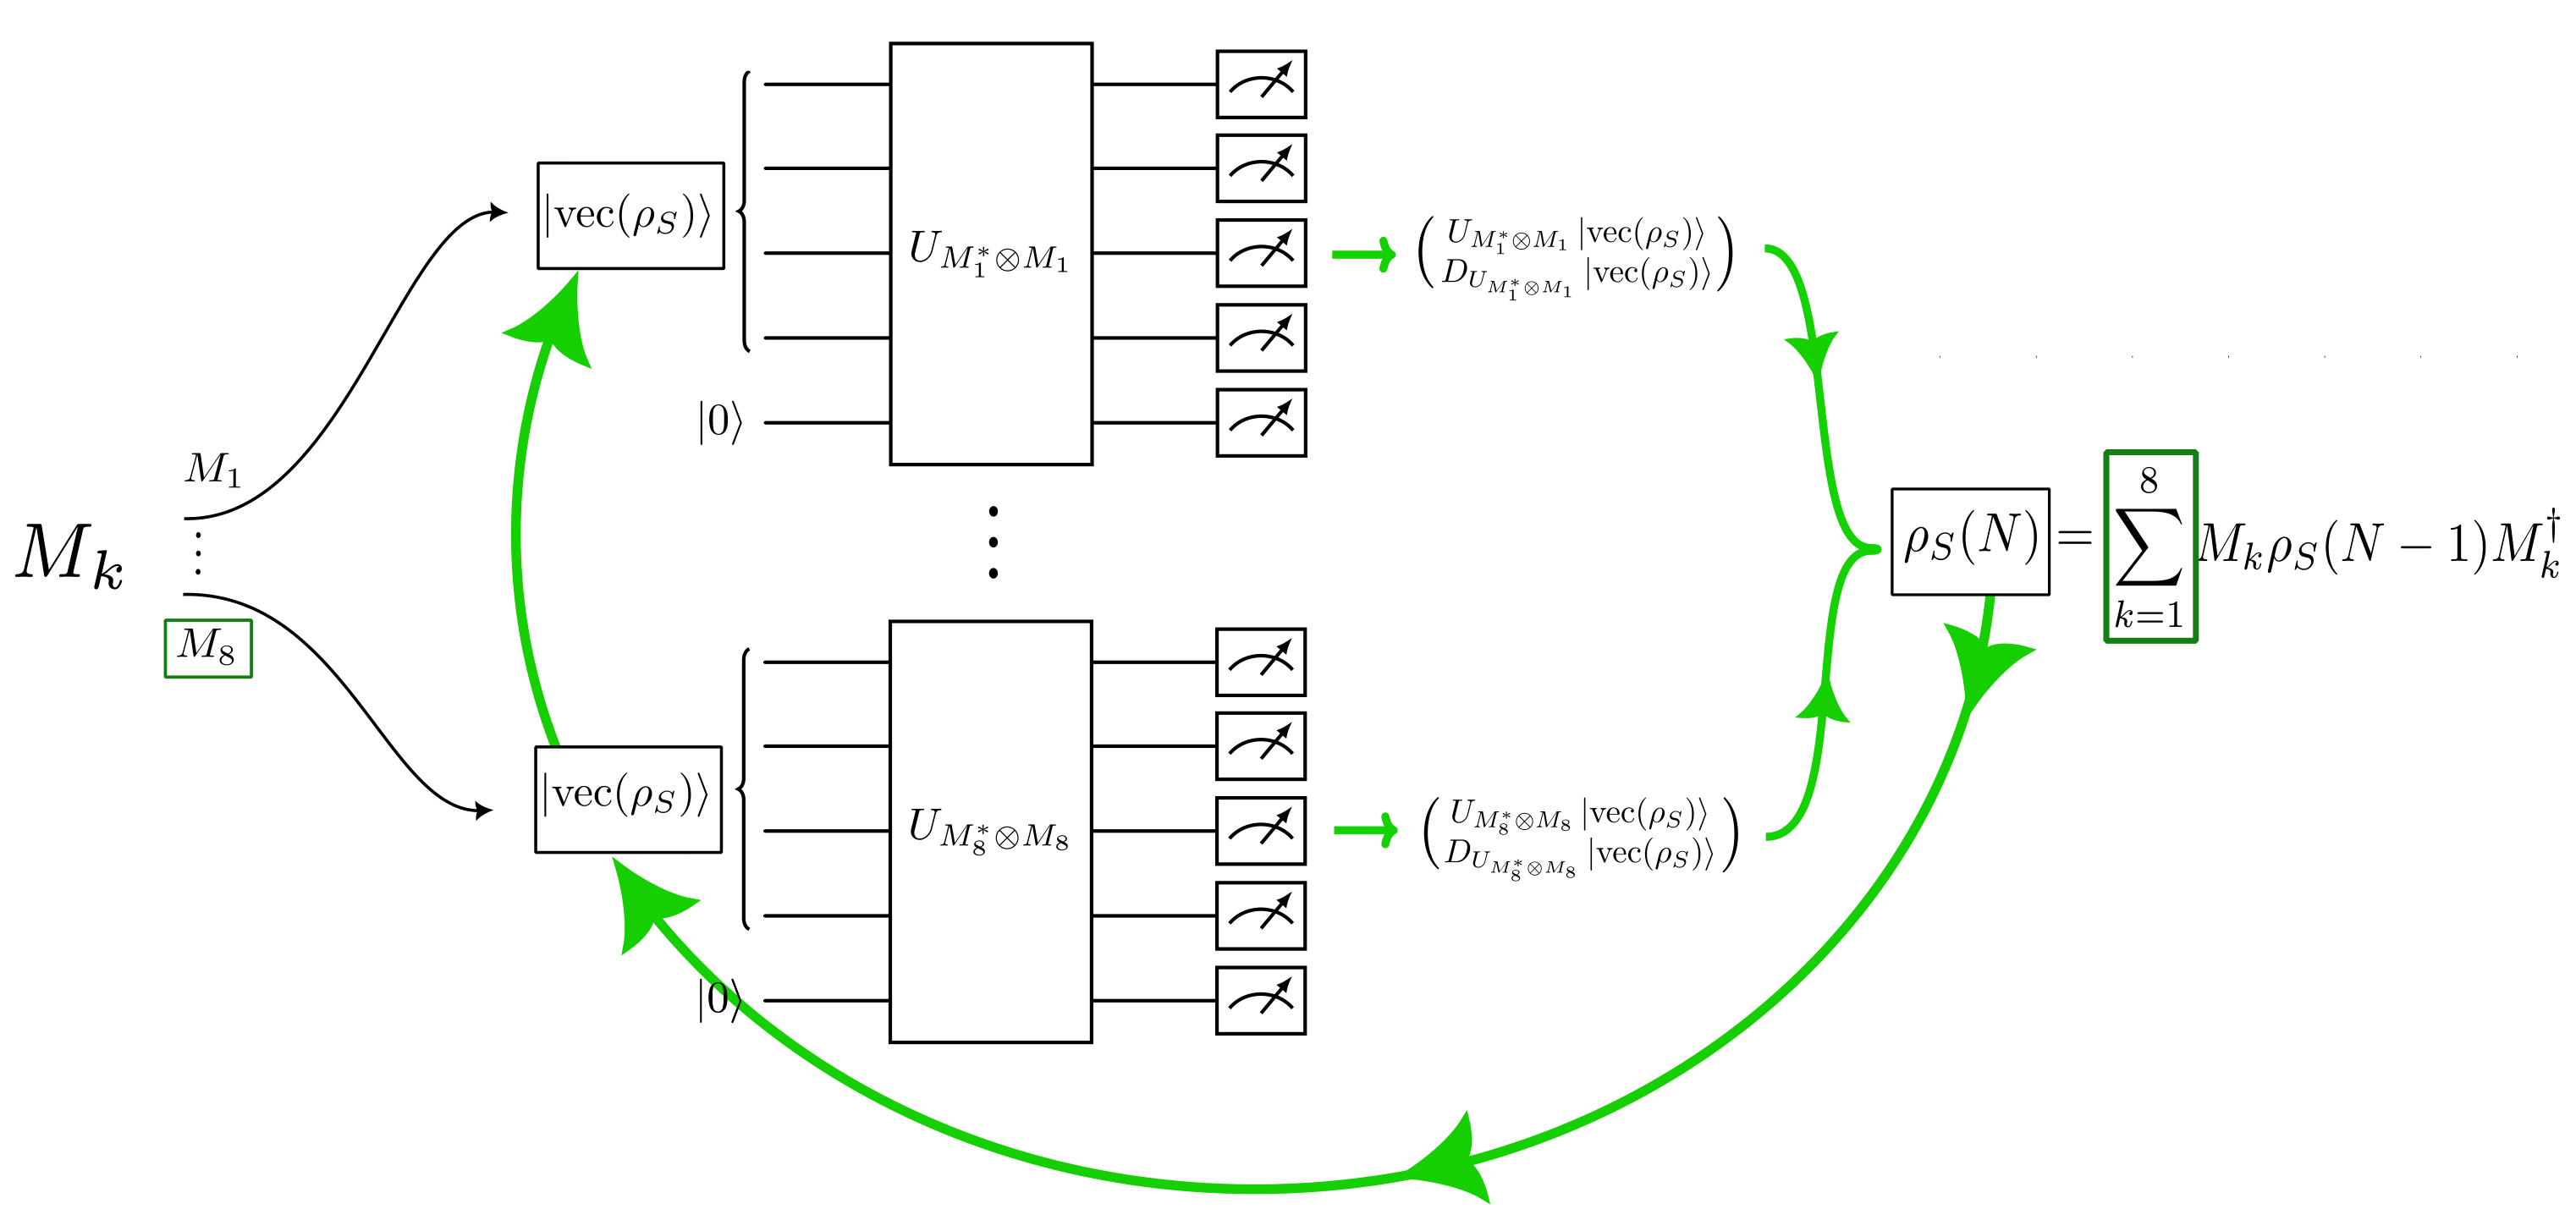
\includegraphics[width=0.92\textwidth]{enh_opsum.png}
\caption{\label{fig:opsum}
The Markovian operator sum on the grid. The one-step map $\Lmap_1$ gives the
Kraus operators $M_1,\dots,M_8$ of the small-step model. Each is dilated to a
unitary $U_{M_k^{*}\otimes M_k}$ and run as one circuit on $\ket{\vecc\rhoS}$,
and the outputs are summed to
$\rhoS(N)=\sum_{k}M_k\,\rhoS(N-1)\,M_k^\dagger$. The result is vectorized and
recycled as the input of the next step along the green loop, so the eight
circuits are constructed a single time and reused. Figure adapted from the
author's master's thesis.}
\end{figure*}

% ==========================================================================
\section{Memory on the register}
\label{sec:memory}
% ==========================================================================
A non-Markovian family cannot be handled this way. Equation~\eqref{eq:markstep}
applies one fixed channel $\Phi$ to the previous state, and iterating it produces
$\Phi^{\,n}$, which is a semigroup by construction. A channel acting on the
system alone therefore reproduces only memoryless dynamics, and every
correlation older than one step is lost. We confirm this failure quantitatively
in Sec.~\ref{sec:results}. The memory has to be represented explicitly, and since
the system channel cannot hold it, we place it on the register.

\subsection{Transfer tensors and the memory window}
The exact dynamics is time nonlocal. Because both the global unitary evolution
and the partial trace are linear in $\rhoS(0)$, the state at step $n$ is a linear
functional of its own past, which the Nakajima-Zwanzig projection makes
precise~\cite{nakajima1958,zwanzig1960}. On the grid this takes the form of a
discrete convolution~\cite{cerrillo2014},
\begin{equation}
  \label{eq:convolution}
  \vecc\!\big(\rhoS(t_n)\big)=\sum_{m=1}^{n} T_m\,\vecc\!\big(\rhoS(t_{n-m})\big),
\end{equation}
where the transfer tensor $T_m$ measures how strongly the state $m$ steps in the
past still acts on the present. Inserting the dynamical maps
$\vecc(\rhoS(t_k))=\Lmap_k\vecc(\rhoS(0))$ and demanding
Eq.~\eqref{eq:convolution} for every initial state gives an operator identity,
$\Lmap_n=\sum_{m=1}^{n}T_m\Lmap_{n-m}$ with $\Lmap_0=\id$, which is solved
recursively (Appendix~\ref{app:ttm}),
\begin{equation}
  \label{eq:ttm}
  T_n=\Lmap_n-\sum_{m=1}^{n-1}T_m\,\Lmap_{n-m}.
\end{equation}
Each step of the recursion removes the part of the dynamics that shorter memories
already account for, so $T_n$ isolates the genuine $n$-step memory. Because the
bath correlations decay, the transfer tensors decay as well, and beyond a memory
time $\tau_{\rm mem}=K\dt$ they are negligible, $T_{m>K}\approx0$. Only the first
$K$ tensors need to be kept, and they are learned from the short-time maps
$\Lmap_1,\dots,\Lmap_K$ alone. This is the central economy of the method. The
classical calculation reaches only the memory window $K\dt$, whereas the earlier
dilation schemes reconstruct an operator for every point of the full
trajectory.

\subsection{The companion operator on the grid}
The convolution~\eqref{eq:convolution} of order $K$ is turned into a first-order
recurrence by enlarging the state. We collect the last $K$ vectorized density
matrices into a sliding window
\begin{equation}
  \label{eq:window}
  X_n=\big(\vecc\rhoS(t_n),\,\vecc\rhoS(t_{n-1}),\,\dots,\,
  \vecc\rhoS(t_{n-K+1})\big)^{T},
\end{equation}
a vector of $K d^2$ entries, and advance it by one fixed operator, $X_{n+1}=E
X_n$, with the block companion matrix
\begin{equation}
  \label{eq:companion}
  E=\begin{pmatrix}
  T_1 & T_2 & \cdots & T_{K-1} & T_K\\
  \id & 0 & \cdots & 0 & 0\\
  0 & \id & \cdots & 0 & 0\\
  \vdots & & \ddots & & \vdots\\
  0 & 0 & \cdots & \id & 0
  \end{pmatrix}.
\end{equation}
Its first block row evaluates the convolution~\eqref{eq:convolution} and writes
the new state into the top slot, while the identity blocks below shift the window
and drop the oldest entry. The operator $E$ is assembled once from the $K$
transfer tensors and is the only object the grid re-applies.

In general $E$ is not a CPTP map, since the individual transfer tensors are not
channels, so the Choi route of the Markovian case does not apply. The Sz.-Nagy
dilation of Eq.~\eqref{eq:sznagy}, with $A=E/s$, needs no such property. It
block-encodes $E$ into one unitary that acts on the window register together with
a single ancilla. On hardware the loop is the same as before. The window is
loaded, the one dilated circuit of Fig.~\ref{fig:circuits} is applied, the
ancilla is post-selected on $\ket{0}$, the top block is read out and rescaled,
and the updated window is fed back. The startup window, for the first $K$ steps,
is taken from the same short-time maps through
$\vecc\rhoS(t_n)=\Lmap_n\vecc\rhoS(0)$. Every step after that is pure prediction
at no further classical cost.

The HEOM family enters this construction through its short-time maps only. The
one matrix exponential $P=e^{\hat{\Ldt}_{\rm HEOM}\dt}$ acts on the auxiliary
hierarchy, not on a density matrix, so it is never the operator the grid reuses.
It is applied once to generate the reduced maps $\Lmap_1,\dots,\Lmap_K$, and
those feed exactly the same transfer tensors, companion operator and dilated
unitary as the path integral. The path integral supplies the same maps directly.

\begin{figure}[t]
\centering
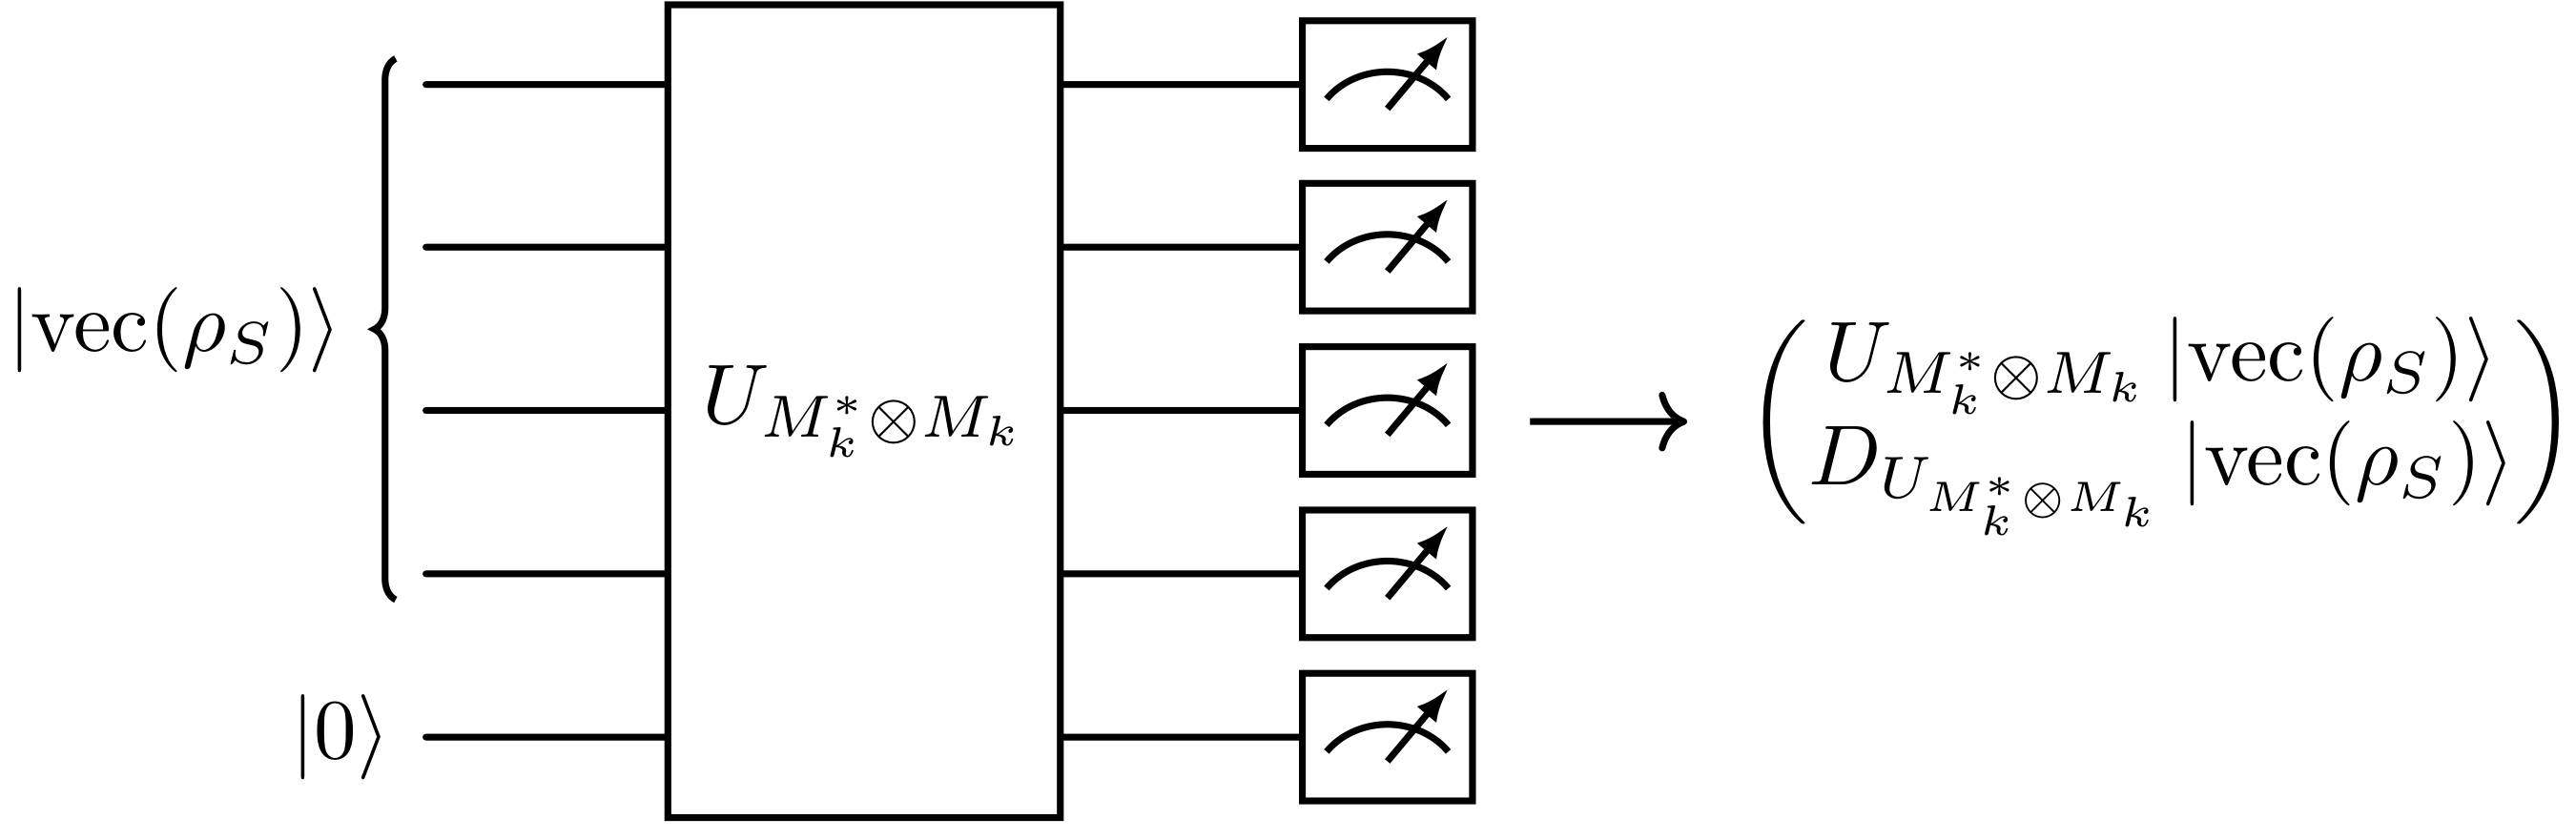
\includegraphics[width=\columnwidth]{enh_circuit.png}
\caption{\label{fig:circuits}
The dilated circuit of one branch. The vectorized density matrix
$\ket{\vecc\rhoS}$ together with one ancilla $\ket{0}$ enters the Sz.-Nagy
dilation $U_{M_k^{*}\otimes M_k}$ of Eq.~\eqref{eq:sznagy}. Post-selecting the
ancilla on $\ket{0}$ leaves $M_k^{*}\otimes M_k\ket{\vecc\rhoS}$ in the system
register, the top block of the output, while the lower block $D$ is the defect
and is discarded. The non-Markovian grid uses the identical construction with
$M_k^{*}\otimes M_k$ replaced by the companion operator $E$ of
Eq.~\eqref{eq:companion} on the window register. Figure adapted from the author's
master's thesis.}
\end{figure}

\begin{figure*}[t]
\centering
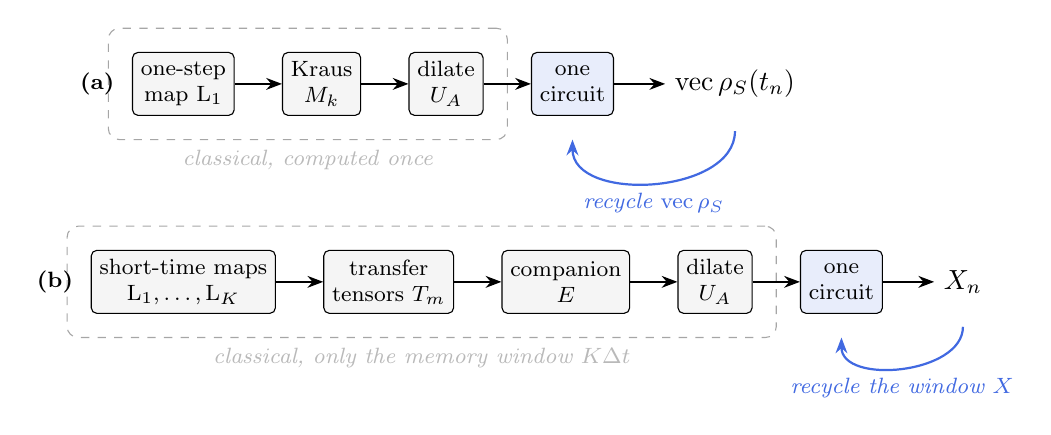
\begin{tikzpicture}[node distance=5.5mm and 6mm]
% (a) Markovian
\node[stage] (l0) {one-step\\map $\Lmap_1$};
\node[stage,right=of l0] (k0) {Kraus\\$M_k$};
\node[stage,right=of k0] (d0) {dilate\\$U_{A}$};
\node[qpu,right=of d0] (q0) {one\\circuit};
\node[right=6.5mm of q0] (o0) {$\vecc\rhoS(t_n)$};
\draw[flow] (l0)--(k0); \draw[flow] (k0)--(d0); \draw[flow] (d0)--(q0);
\draw[flow] (q0)--(o0);
\begin{scope}[on background layer]
\node[draw,dashed,Gray!70,rounded corners,fit=(l0)(d0),inner sep=3mm,
  label={[font=\footnotesize\itshape,Gray!55]below:classical, computed once}]{};
\end{scope}
\draw[recyc] ([yshift=-3mm]o0.south) to[out=-90,in=-90]
  node[below,font=\footnotesize\itshape,RoyalBlue]{recycle $\vecc\rhoS$}
  ([yshift=-3mm]q0.south);
\node[left=1mm of l0,font=\footnotesize\bfseries] {(a)};
% (b) non-Markovian
\node[stage,below=17mm of l0] (l1) {short-time maps\\$\Lmap_1,\dots,\Lmap_K$};
\node[stage,right=of l1] (t1) {transfer\\tensors $T_m$};
\node[stage,right=of t1] (c1) {companion\\$E$};
\node[stage,right=of c1] (d1) {dilate\\$U_{A}$};
\node[qpu,right=of d1] (q1) {one\\circuit};
\node[right=6.5mm of q1] (o1) {$X_n$};
\draw[flow] (l1)--(t1); \draw[flow] (t1)--(c1); \draw[flow] (c1)--(d1);
\draw[flow] (d1)--(q1); \draw[flow] (q1)--(o1);
\begin{scope}[on background layer]
\node[draw,dashed,Gray!70,rounded corners,fit=(l1)(d1),inner sep=3mm,
  label={[font=\footnotesize\itshape,Gray!55]below:classical, only the memory window $K\dt$}]{};
\end{scope}
\draw[recyc] ([yshift=-3mm]o1.south) to[out=-90,in=-90]
  node[below,font=\footnotesize\itshape,RoyalBlue]{recycle the window $X$}
  ([yshift=-3mm]q1.south);
\node[left=1mm of l1,font=\footnotesize\bfseries] {(b)};
\end{tikzpicture}
\caption{\label{fig:schematic}
The two variants of the grid. (a) A Markovian (semigroup) family needs only the
one-step map. Its Kraus operators are dilated once and the circuit is re-applied,
recycling the vectorized density matrix. (b) A non-Markovian family is learned on
the memory window $K\dt$. The short-time maps give the transfer tensors, which
build the companion operator $E$. Its dilation is the reused circuit, which
advances the sliding window $X$. In both variants the classical work is done
once, and the quantum device carries the propagation.}
\end{figure*}

% ==========================================================================
\section{Results for the FMO complex}
\label{sec:results}
% ==========================================================================
We take the dominant $1\to2\to3\to4$ transfer pathway of the FMO complex defined
by the model of Sec.~\ref{sec:map}, with a time step $\dt=10$~fs and the initial
excitation on site 1. The Lindblad family uses a secular Redfield generator, the
HEOM family a hierarchy of depth three, and the path integral the TEMPO
contraction with an SVD cutoff of $10^{-6}$. The transfer tensors decay within a
memory window of $K=15$ steps ($150$~fs) for the path integral and $K=25$ steps
($250$~fs) for the HEOM maps.

Figure~\ref{fig:grid} shows the populations of all four sites to $1000$~fs. The
three colored curves are produced entirely on the reused dilated circuit, the
Lindblad map through the one-step Kraus operators and the HEOM and path-integral
maps through the companion operator. They lie on top of the numerically exact
solvers, drawn as dashed lines. The dotted vertical lines mark the two memory
windows. To their left the circuit is still primed with the learned short-time
maps. Everything to their right is generated by the quantum device alone, and it
continues to track the exact dynamics for the remaining $750$ to $850$~fs at no
further classical cost. The non-Markovian curves, path integral and HEOM, keep
the pronounced early oscillations that signal the backflow of information from
the bath, while the Markovian Lindblad curve relaxes monotonically, so the
memory that the register carries is physically visible.

\begin{figure}[t]
\centering
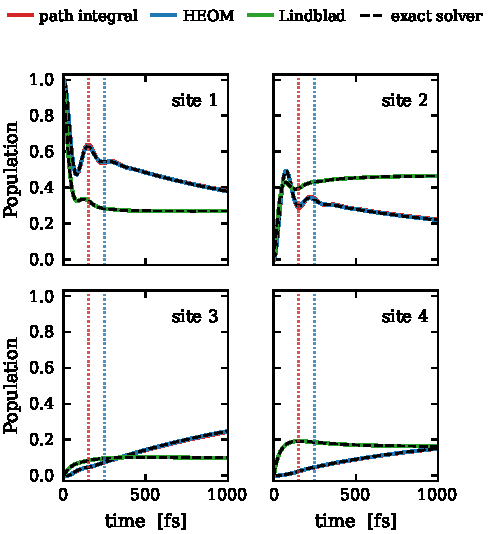
\includegraphics[width=\columnwidth]{fig_grid.pdf}
\caption{\label{fig:grid}
FMO populations produced on one reused dilated circuit for the three maps,
against the numerically exact solvers (dashed). The dotted vertical lines mark
the memory windows $K\dt$, at $150$~fs for the path integral and $250$~fs for
HEOM. To the right of each line the quantum device propagates on its own, with no
further classical input, and still reproduces the exact dynamics. Colors label
the three methods.}
\end{figure}

The transfer tensors also measure the non-Markovianity directly. For a semigroup
$\Lmap_n=\Lmap_1^{\,n}$ the recursion~\eqref{eq:ttm} gives $T_m=0$ for $m\ge2$,
so a memoryless process has a single nonzero tensor. Figure~\ref{fig:memory}(a)
confirms this for the Lindblad family, whose tensors collapse to machine
precision beyond the first, while the HEOM and path-integral tensors remain
finite and decay by about two orders of magnitude across the window. That decay
is what sets the window size and controls the truncation.
Figure~\ref{fig:memory}(b) shows how the accuracy improves as the window grows.
A longer window lowers the error until it saturates, at about $10^{-2}$ for the
path integral, which is the accuracy of the path-integral map against the HEOM
reference, and near $2\times10^{-4}$ for the HEOM maps against their own solver.

\begin{figure}[t]
\centering
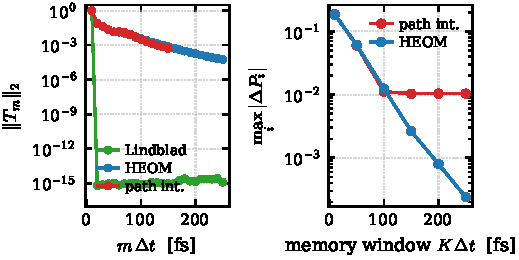
\includegraphics[width=\columnwidth]{fig_memory.pdf}
\caption{\label{fig:memory}
(a) Norm of the transfer tensors $\|T_m\|_2$ against the delay $m\dt$. For the
Markovian Lindblad family every tensor beyond the first vanishes to machine
precision, the exact signature of a memoryless semigroup. For the HEOM and
path-integral families the tensors are nonzero and decay by about two orders of
magnitude across the window, which both measures the non-Markovian memory and
controls its truncation at $K$. (b) Maximum population error against the memory
window $K\dt$. The error falls as the window lengthens and then saturates at the
accuracy of the underlying map.}
\end{figure}

That the memory is essential, and not a refinement, is shown in
Fig.~\ref{fig:deviation}. It plots the deviation of each grid result from the
exact solver. The Lindblad case is reproduced to machine precision, since its
family is a genuine semigroup and one step is exact. The HEOM and path-integral
cases stay at the accuracy of their maps once the window is in place, near
$2\times10^{-4}$ and $10^{-2}$. The gray curve applies the memoryless variant,
$K=1$, to the path-integral map. It discards every correlation beyond one step
and its error rises to about $0.2$, an error of order one on populations bounded
by unity. The memory window is therefore what turns the reused circuit into a
faithful non-Markovian propagator.

\begin{figure}[t]
\centering
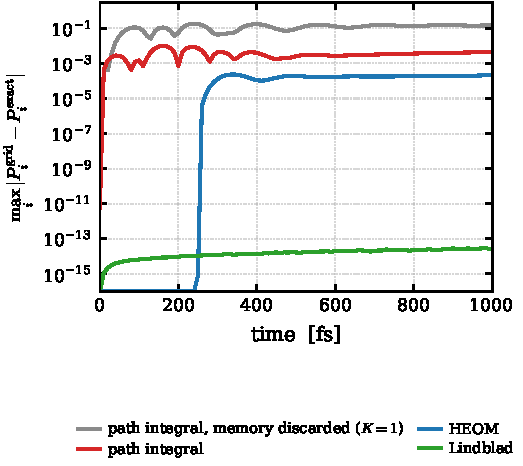
\includegraphics[width=\columnwidth]{fig_deviation.pdf}
\caption{\label{fig:deviation}
Deviation of the grid result from the exact solver. Lindblad is reproduced to
machine precision. HEOM and the path integral stay at the accuracy of their maps.
Discarding the memory, the $K=1$ variant applied to the path-integral map (gray),
raises the error to order one, which shows that the memory window is essential.}
\end{figure}

Two properties confirm that the reused circuit is a valid propagator and not
merely an accurate fit. The first is stability. The companion operator $E$ drives
the whole non-Markovian trajectory through $X_{n+1}=EX_n$, so a spectral radius
above one would make the prediction diverge. Figure~\ref{fig:validity}(a) shows
that every eigenvalue of $E$ lies in the closed unit disk, for both the HEOM and
the path-integral maps. The steady state sits at the marginal eigenvalue
$\lambda=1$ and all other modes decay, so the recurrence is Schur stable and the
trajectory stays bounded for any number of steps. The second is physicality.
Although the transfer tensors and $E$ are not themselves completely positive, the
matrix they produce remains a density matrix. Figure~\ref{fig:validity}(b) shows
that the trace is conserved to between $10^{-11}$ and $10^{-5}$ across the full
propagation, and the smallest eigenvalue of $\rhoS(t)$ never drops below
$-10^{-11}$, so the state stays positive. The grid respects the two defining
constraints of a density matrix while it predicts.

\begin{figure}[t]
\centering
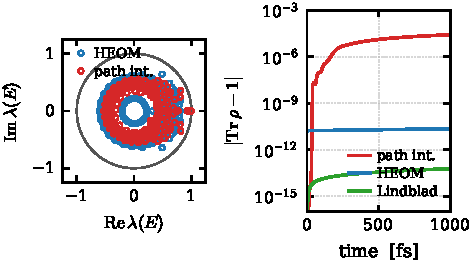
\includegraphics[width=\columnwidth]{fig_validity.pdf}
\caption{\label{fig:validity}
Validity of the memory-window grid. (a) Eigenvalues of the companion operator $E$
for the HEOM and path-integral maps. All lie in the closed unit disk, with the
steady state at the marginal $\lambda=1$ and every other mode inside, so the
recurrence $X_{n+1}=EX_n$ is stable. (b) The trace of the propagated density
matrix is conserved throughout, and its smallest eigenvalue stays above
$-10^{-11}$, so the state remains physical.}
\end{figure}

The register grows with the window. The Markovian circuit uses five qubits, four
for $\vecc(\rhoS)$ and one ancilla. The non-Markovian window register holds $K
d^2$ amplitudes, padded to the next power of two, so the path integral with
$K=15$ uses nine qubits and the HEOM maps with $K=25$ use ten. This is the price
of carrying the memory, and it is a fixed cost set by the memory time rather than
by the length of the propagation. The decisive point is the split of labor. The
classical computer produces $K$ short-time maps, once, and the quantum device
then generates a trajectory of arbitrary length by re-applying a single circuit.

% ==========================================================================
\section{Outlook}
\label{sec:outlook}
% ==========================================================================
The grid moves the propagation onto the quantum processor and creates one
genuinely quantum demand. To feed the state back, the register must be read out
after each step, its amplitudes together with its phases. A projective
measurement returns only populations, so the full state has to be reconstructed
by quantum tomography, and the reconstruction has to be accurate enough that the
error does not accumulate as it is recycled. The window register makes this the
principal cost, because its size grows with the memory time, and the ancilla
post-selection of the dilation succeeds only with a probability that sets the
number of shots.

Scalable state estimation is therefore the natural next step. Classical shadows
predict many observables from a number of randomized measurements that grows only
logarithmically in the number of target properties~\cite{huang2020}.
Compressed-sensing tomography exploits that the recycled state is close to pure,
so a density matrix of dimension $d$ and rank $r$ is recovered from about
$\mathcal{O}(rd\log^2 d)$ settings~\cite{gross2010}. Neural-network tomography
compresses the state into a generative model trained from a modest set of
snapshots and has reconstructed highly entangled states of many
qubits~\cite{torlai2018}. Folding any of these into the recycling loop, so that a
compact and noise-robust description of the window is propagated, is in our view
the step that would turn the memory-window grid into a practical tool for
non-Markovian simulation on quantum hardware.

% ==========================================================================
\section{Conclusion}
\label{sec:conclusion}
% ==========================================================================
We have organized the quantum simulation of open-system dynamics around one idea.
The dynamical map is turned once into a single dilated circuit, and the quantum
computer generates the trajectory by re-applying it. For a Markovian map the
semigroup property makes one one-step operator sufficient. For a non-Markovian
map, where a system channel cannot hold the memory, we place the memory on the
register. The exact dynamics is a discrete convolution over transfer tensors that
decay within a finite window, so only the tensors of that window are learned,
packed into one companion operator, and dilated into the reused circuit. The
classical cost is then set by the memory time and not by the length of the
propagation. On a four-site FMO pathway the scheme reproduces the numerically
exact dynamics to 1000 fs, for the Lindblad, HEOM and path-integral maps alike,
from a memory window of 150 to 250 fs, while discarding the memory raises the
error to order one. The remaining obstacle is the read-out of the window for the
recycling step, for which scalable estimators are the most promising route. The
memory-window grid brings the bulk of a non-Markovian open-system simulation onto
the quantum device.

\begin{acknowledgments}
This work builds on the master's thesis of S.M. at the Institute for Theoretical
Physics, Johannes Kepler University Linz. The three dynamical maps were
implemented independently and cross-validated against the qutip solvers.
\end{acknowledgments}

\appendix

% ==========================================================================
\section{Vectorization, the Liouvillian, and the Choi-Kraus construction}
\label{app:vec}
% ==========================================================================
\emph{Vectorization.} Column stacking sends a $d\times d$ matrix $\rhoS$ to the
length-$d^2$ vector $\vecc(\rhoS)$ with entries $\vecc(\rhoS)_{i+dj}=(\rhoS)_{ij}$,
and obeys the identity
\begin{equation}
  \label{eq:vecid}
  \vecc(ABC)=(C^{T}\otimes A)\,\vecc(B).
\end{equation}
Setting $B=\rhoS$ and taking $A$ or $C$ equal to the identity turns any left or
right multiplication into a matrix acting on $\vecc(\rhoS)$, which is what turns
each dynamical map $\Emap_n$ into the matrix $\Lmap_n$ of Eq.~\eqref{eq:vecmap}.

\emph{The Lindblad generator.} Applied to the Lindblad master
equation~\cite{lindblad1976,gks1976}
\begin{equation}
  \dv{\rhoS}{t}=-\tfrac{i}{\hbar}[H_S,\rhoS]+\sum_\alpha\gamma_\alpha\Big(L_\alpha\rhoS L_\alpha^\dagger-\tfrac12\{L_\alpha^\dagger L_\alpha,\rhoS\}\Big),
\end{equation}
Eq.~\eqref{eq:vecid} gives $\dv{}{t}\vecc(\rhoS)=\Ldt\vecc(\rhoS)$ with the time
independent generator
\begin{equation}
\begin{split}
  \Ldt=&-\tfrac{i}{\hbar}\big(\id\otimes H_S-H_S^{T}\otimes\id\big)\\
  &+\sum_\alpha\gamma_\alpha\Big(L_\alpha^{*}\!\otimes\! L_\alpha
  -\tfrac12\id\otimes L_\alpha^\dagger L_\alpha-\tfrac12 L_\alpha^{T}L_\alpha^{*}\!\otimes\!\id\Big),
\end{split}
\end{equation}
where the commutator produces the first two terms through
$\vecc(H_S\rhoS)=(\id\otimes H_S)\vecc\rhoS$ and
$\vecc(\rhoS H_S)=(H_S^{T}\otimes\id)\vecc\rhoS$, and each dissipator term uses
$(L_\alpha^\dagger)^{T}=L_\alpha^{*}$. Because $\Ldt$ is constant,
$\Lmap_n=e^{\Ldt t_n}=\Lmap_1^{\,n}$, a semigroup.

\emph{Choi and Kraus.} The Kraus operators of a map $\Lmap$ follow from its Choi
matrix~\cite{choi1975}
\begin{equation}
  \mathcal{C}=\sum_{i,j=1}^{d}E_{ij}\otimes\Lmap[E_{ij}],\qquad
  \Lmap[E_{ij}]=\mathrm{unvec}(\Lmap\,\vecc E_{ij}),
\end{equation}
with $E_{ij}$ the matrix units. Choi's theorem states that $\Lmap$ is completely
positive if and only if $\mathcal{C}\succeq0$. The eigendecomposition
$\mathcal{C}=\sum_k\sigma_k u_k u_k^\dagger$ with $\sigma_k\ge0$ then gives
$\vecc(M_k)=\sqrt{\sigma_k}\,u_k$, which rebuilds
$\rhoS=\sum_k M_k\rhoS(0)M_k^\dagger$ and confirms Eq.~\eqref{eq:markstep}. Trace
preservation is the condition $\sum_k M_k^\dagger M_k=\id$, equivalently
$\id^{T}\Lmap=\id^{T}$ in Liouville space. We take the smallest eigenvalue of
$\mathcal{C}$ as a diagnostic of complete positivity. For the three families it
stays above $-2\times10^{-10}$ across the full propagation, so the maps are CP to
numerical precision and the operator sum is well defined.

% ==========================================================================
\section{Construction of the three dynamical maps}
\label{app:maps}
% ==========================================================================
Each method returns the same object, the family $\{\Lmap_n\}$ of
Eq.~\eqref{eq:vecmap}, but reaches it differently. In every case the bath enters
only through the correlation function $C(\tau)$ of Eq.~\eqref{eq:Ctau}.

\subsection{Secular Redfield}
The system-bath coupling is $H_{SB}=\sum_m A_m\otimes B_m$ with the site
projectors $A_m=\dyad{m}$. In the eigenbasis $H_S=\sum_a\varepsilon_a\dyad{a}$
each coupling operator resolves into eigenoperators at the Bohr frequencies
$\omega=(\varepsilon_b-\varepsilon_a)/\hbar$,
\begin{equation}
  \label{eq:eigenop}
  A_m(\omega)=\!\!\sum_{\varepsilon_b-\varepsilon_a=\hbar\omega}\!\!\bra{a}A_m\ket{b}\,\dyad{a}{b}.
\end{equation}
In the Born-Markov and secular approximation the generator takes the Lindblad
form~\cite{breuer2002}
\begin{equation}
  \label{eq:redfield}
  \begin{split}
  \Ldt[\rhoS]=&-\tfrac{i}{\hbar}[H_S+H_{\rm LS},\rhoS]\\
  &+\sum_m\sum_\omega\gamma_m(\omega)\Big(A_m(\omega)\rhoS A_m^\dagger(\omega)\\
  &\qquad\quad-\tfrac12\big\{A_m^\dagger(\omega)A_m(\omega),\rhoS\big\}\Big),
  \end{split}
\end{equation}
with a Lamb shift $H_{\rm LS}$ and rates fixed by the full Fourier transform of
the correlation function,
\begin{equation}
  \label{eq:rate}
  \gamma_m(\omega)=\int_{-\infty}^{\infty}\!d\tau\,e^{i\omega\tau}\,C(\tau),
  \qquad \gamma(-\omega)=e^{-\beta\hbar\omega}\gamma(\omega),
\end{equation}
the second relation being detailed balance. Comparison with
Appendix~\ref{app:vec} identifies the jump operators $L_\alpha=A_m(\omega)$ and
the rates $\gamma_\alpha=\gamma_m(\omega)$, so the family is completely positive
and a semigroup.

\subsection{Hierarchical equations of motion}
For the Drude spectral density~\eqref{eq:J} the correlation function
$C(\tau)$ of Eq.~\eqref{eq:Ctau} decomposes into a Drude pole and Matsubara
terms,
\begin{equation}
  \label{eq:cexp}
  C(\tau)=\sum_{k\ge0}c_k\,e^{-\nu_k\tau},
\end{equation}
which in the convention $\hbar=1$ used here carry the coefficients
\begin{equation}
  \label{eq:matsubara}
  \begin{aligned}
  &\nu_0=\gamma, & &c_0=\lambda\gamma\big[\cot\tfrac{\beta\gamma}{2}-i\big],\\
  &\nu_k=\tfrac{2\pi k}{\beta}, & &c_k=\tfrac{4\lambda\gamma}{\beta}\,\frac{\nu_k}{\nu_k^2-\gamma^2}\ \ (k\ge1),
  \end{aligned}
\end{equation}
truncated after a few Matsubara terms. Each exponential $k$ carries one index
$n_k$ of the multi-index $\bm n$, and the auxiliary operators $\rho_{\bm n}$ obey
the hierarchy~\eqref{eq:heom}, which couples $\bm n$ to its neighbors
$\bm n_k^\pm$. Truncating the depth at $\sum_k n_k\le n_{\max}$ closes the set,
and stacking $\{\rho_{\bm n}\}$ into one supervector turns the right hand side
into a constant generator $\hat\Ldt_{\rm HEOM}$, so that
$P=e^{\hat\Ldt_{\rm HEOM}\dt}$ advances the whole hierarchy by one step. The
reduced map is read from the physical tier,
\begin{equation}
  \label{eq:heomextract}
  \Lmap_n\,\vecc(E_{ij})=\vecc\Big(\big[\,P^{\,n}\,(E_{ij}\oplus 0)\,\big]_{\bm 0}\Big),
\end{equation}
by propagating each basis matrix $E_{ij}$ with vanishing auxiliaries and keeping
the physical tier $\rho_{\bm 0}$. We use $n_{\max}=3$.

\subsection{Tensor-network path integral}
On the discretized contour of spacing $\dt$ each branch is a string of site
labels $s_0^\pm,\dots,s_N^\pm$, and the bare evolution across one slice is the
short-time system propagator
\begin{equation}
  \label{eq:shorttime}
  K_{s s'}=\bra{s}e^{-iH_S\dt/\hbar}\ket{s'}.
\end{equation}
The path integral~\eqref{eq:pathint} then reduces to a sum over these labels,
weighted by the forward and backward propagators and by the influence
functional~\eqref{eq:influence}, whose coefficients are the double slice integrals
\begin{equation}
  \label{eq:eta}
  \eta_{kk'}=\int_{k\dt}^{(k+1)\dt}\!\!dt\int_{k'\dt}^{(k'+1)\dt}\!\!dt'\;C(t-t'),
\end{equation}
evaluated in closed form for the exponential representation~\eqref{eq:cexp} of
$C(\tau)$. Collecting the labels at each time into one augmented index and the
pairwise weights into a tensor gives the TEMPO network, contracted as a matrix
product state with a singular-value cutoff of $10^{-6}$~\cite{strathearn2018,bose2022}.
The reduced density matrix at step $n$ is the contraction
\begin{equation}
  \label{eq:pinet}
  \big[\rhoS(t_n)\big]_{s_n^+ s_n^-}=\!\!\sum_{\{s_k^\pm\}_{0\le k<n}}\!\!
  W^{(n)}_{\{s^\pm\}}\;\big[\rhoS(0)\big]_{s_0^+ s_0^-},
\end{equation}
with $W^{(n)}$ the accumulated propagator and influence weight. Leaving the
initial pair $(s_0^+,s_0^-)$ open rather than summed identifies the columns of
$\Lmap_n$, so a single contraction returns the whole map. The bath memory is
truncated at the same window $K$ that later bounds the transfer tensors.

% ==========================================================================
\section{Transfer tensors, the companion operator, and stability}
\label{app:ttm}
% ==========================================================================
\emph{Memory kernel.} The Nakajima-Zwanzig projection~\cite{nakajima1958,zwanzig1960}
separates the Liouville-von Neumann dynamics into a relevant system part and an
irrelevant bath part and produces a closed but time-nonlocal equation for the
reduced state, driven by a memory kernel. Its discrete-time counterpart is the
convolution~\eqref{eq:convolution}, in which the transfer tensor $T_m$ is the
kernel integrated over the $m$th slice~\cite{cerrillo2014}. Because both the
global unitary evolution and the partial trace are linear in $\rhoS(0)$, the
tensors are state independent.

\emph{Recursion.} Substituting $\vecc\rhoS(t_k)=\Lmap_k\vecc\rhoS(0)$ into
Eq.~\eqref{eq:convolution} and demanding it for every initial state gives the
operator identity $\Lmap_n=\sum_{m=1}^{n}T_m\Lmap_{n-m}$ with $\Lmap_0=\id$.
Isolating the $m=n$ term yields Eq.~\eqref{eq:ttm},
$T_n=\Lmap_n-\sum_{m=1}^{n-1}T_m\Lmap_{n-m}$. For a semigroup
$\Lmap_n=\Lmap_1^{\,n}$ one finds $T_1=\Lmap_1$ and, by induction, $T_n=0$ for
$n\ge2$, so a single tensor carries all Markovian dynamics. For a non-Markovian
family the tensors decay with the bath correlations and are truncated at the
window $K$. They are closely related to the memory kernel of a discretized
process tensor~\cite{pollock2018,jorgensen2019}.

\emph{Companion operator.} The window $X_n$ of Eq.~\eqref{eq:window} stacks the
last $K$ states. The companion matrix $E$ of Eq.~\eqref{eq:companion} satisfies
$X_{n+1}=EX_n$. Its first block row evaluates
$\sum_{m=1}^{K}T_m\vecc\rhoS(t_{n+1-m})$, which is the new state by
Eq.~\eqref{eq:convolution}, while each identity block below copies one entry of
the window down by one slot and the oldest entry is dropped. The operator $E$ is
thus assembled once from the $K$ transfer tensors and encodes the whole memory.

\emph{Dilation.} The individual transfer tensors are not channels, so $E$ is
generally not completely positive and the Choi route does not apply. Instead
$E/s$ with $s\ge\|E\|_2$ is a contraction and is block-encoded by the Sz.-Nagy
dilation of Eq.~\eqref{eq:sznagy}, in which $B=(\id-AA^\dagger)^{1/2}$ and
$C=(\id-A^\dagger A)^{1/2}$ with $A=E/s$. One checks $U_A^\dagger U_A=\id$ directly
from these definitions. Preparing $\ket{0}_{\rm anc}\otimes\ket{X_n}$, applying
$U_A$ and post-selecting the ancilla on $\ket{0}$ leaves $A\ket{X_n}$ in the
register, and multiplying by $s$ returns $EX_n$. The startup window uses
$\vecc\rhoS(t_n)=\Lmap_n\vecc\rhoS(0)$ for $n<K$ from the short-time maps.

\emph{Stability.} The propagation is stable because the spectral radius of $E$
does not exceed one. Trace preservation of the underlying maps forces a marginal
eigenvalue at $\lambda=1$, whose eigenvector is the fixed point of the window,
namely the steady state repeated $K$ times. Every other eigenvalue lies inside
the unit disk and corresponds to a decaying mode, as Fig.~\ref{fig:validity}(a)
shows. Iterating $E$ therefore neither amplifies nor suppresses the physical
state, and the reused circuit propagates for any number of steps without drift.

% ==========================================================================
\section{Comparison with earlier dilation schemes}
\label{app:compare}
% ==========================================================================
Table~\ref{tab:compare} sets the grid beside the schemes it builds on.
Seneviratne \textit{et al.}~\cite{seneviratne2024} propagate the wavefunction and
reach shallow circuits with a singular value decomposition and Walsh operators,
but they rebuild the Kraus operators for every output time, so the classical
effort grows with the length of the propagation. Hu \textit{et
al.}~\cite{hu2022} propagate over small Trotter steps and dilate with the
Sz.-Nagy construction, but composing the single-step operators to reach step $N$
produces $8^{N}$ terms for the eight-operator model, which confines the scheme to
short times. A recent HEOM-based approach~\cite{dan2025} computes the
non-Markovian propagator on the classical computer, so no quantum advantage
remains. The grid keeps the dilation of these schemes but reuses one operator.
For a Markovian map that operator is the one-step channel. For a non-Markovian map
it is the companion operator learned on the memory window, and the classical cost
is set by that window rather than by the number of steps.

\begin{table*}[t]
\caption{\label{tab:compare}
The memory-window grid beside the dilation schemes it builds on. Here $d$ is the
system dimension, $N$ the number of steps, and $K$ the memory window.}
\begin{ruledtabular}
\begin{tabular}{llll}
 & Seneviratne \textit{et al.}~\cite{seneviratne2024}
 & Hu \textit{et al.}~\cite{hu2022}
 & This work (grid) \\
\colrule
Dynamics covered      & Markovian and non-Markovian & Markovian & Markovian and non-Markovian \\
Propagated object     & wavefunction $\ket{\psi}$   & wavefunction $\ket{\psi}$ & density matrix $\vecc\rhoS$, or window $X$ \\
Reused operator       & none, rebuilt each time     & none, composed each step & one-step channel, or companion $E$ \\
Memory                & from the map, per time      & one Trotter step & memory window $K\dt$, on the register \\
Dilation              & SVD with Walsh operators    & Sz.-Nagy & Sz.-Nagy \\
Classical cost        & order $N$ maps              & order $8^{N}$ terms & order $K$ maps \\
Quantum propagation   & one time per output         & bounded by term growth & arbitrary length, one reused circuit \\
Principal limitation  & classical, grows with $N$   & exponential term growth & read-out of the window \\
\end{tabular}
\end{ruledtabular}
\end{table*}

\bibliographystyle{apsrev4-2}
\bibliography{references}

\end{document}
